\title{Riassunto Network Security and Management}
\author{
        Tommaso Puccetti \\
                Studente presso Universita degli studi di Firenze
}
\date{\today}

\documentclass[12pt]{article}
\usepackage{graphicx}
\usepackage{hyperref}

\begin{document}
	
	\maketitle
	\tableofcontents
	\listoftables
	\listoffigures
	
	\section{Security Basics}
		Proprietà della \textbf{Security}:
		\begin{itemize}
			\item \textbf{Confidentiality:} assicurare che persone non autorizzate accedano alle informazioni.
			\item \textbf{Integrity:} assicurare che le informazioni non vengano alterate da individui non autorizzati, in un modo che non sia individuabile dagli utenti autorizzati
			\item \textbf{Authentication}: Assicurarsi che gli utenti siano chi  dicono di essere.
		\end{itemize}
		La security non deve essere confusa con la sicurezza. \textbf{Security:}
		\begin{itemize}
			\item La qualità o lo stato di essere sicuri (liberi da pericoli, da paura o ansi, libero dalla prospettiva di essere licenziato);
			\item Qualcosa di dato, depositato o impegnato con lo scopo di rendere un impegno un obbligo;
			\item Uno strumento di investimento nella forma di un contratto, che fornisce l'evidenza della sua proprietà;
			\item Qualcosa che protegge (misure messe in atto contro lo spionaggio o sabotaggio, crimini o attacchi.)
		\end{itemize}
		Per quanto riguarda la safety:
		\begin{itemize}
			\item La condizione di essere sicuri rispetto al subire o causare danno, infortuni, o perdite.
			\item Un dispositivo progettato per prevenire operazione involontarie o pericolose.	
		\end{itemize}
		La sicurezza ha un \textbf{costo}: un sistema sicuro è \textbf{più complesso da realizzare e da manutenere}, in definitiva \textbf{più complesso}. BLABLABLA
		
	\section{NAT}
		\textbf{Problema}: \textit{gli indirizzi IP sono pochi e costosi, per di più non sempre vogliamo esporre la struttura interna di una Intranet (rete locale)}.\\
		Pe questo motivo vengono utilizzate classi di indirizzi IP (IPv4) \textbf{non-routable} come definito in \textbf{RFC 1918}, riservati alle reti locali con lo \textbf{scopo di ridurre le richieste su indirizzi pubblici}. I pacchetti con tali indirizzi per l'instradamento e l'indirizzamento tramite protocollo IP da router internet.\\
		Si utilizza il \textbf{NAT} e \textbf{NAPT} mascherano un indirizzo tramite proxy a livello IP:
		\begin{itemize}
			\item Si trasforma un indirizzo sorgente (IP Number e port) in un altro indirizzo.
			\item Il server NAT viene visto all'esterno come la sorgente della comunicazione
			\item Il NAT è \textbf{trasparente} per l'utente interno 
		\end{itemize}
		
		\textit{Classi di indirizzi privati:\ref{fig:1}}
		\begin{figure}[h!]
			\centering
			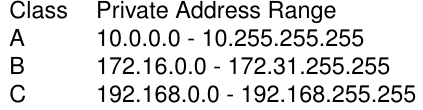
\includegraphics[scale=0.40]{img/class.PNG}
			\caption{Security concepts and relationships\label{fig:1}}
		\end{figure}
		
		\subsection{NAT statico}
			\begin{itemize}
				\item Si ha un mapping uno a uno tra indirizzi esterni ed interni.
				\item Può essere utilizzato in congiunzione con un firewall.
				\item Non risolve il problema della scarsità di indirizzi.
				\item Risulta molto facile da implementare	
			\end{itemize}
		
		\textit{NAT Statico:\ref{fig:2}}
		\begin{figure}[h!]
			\centering
			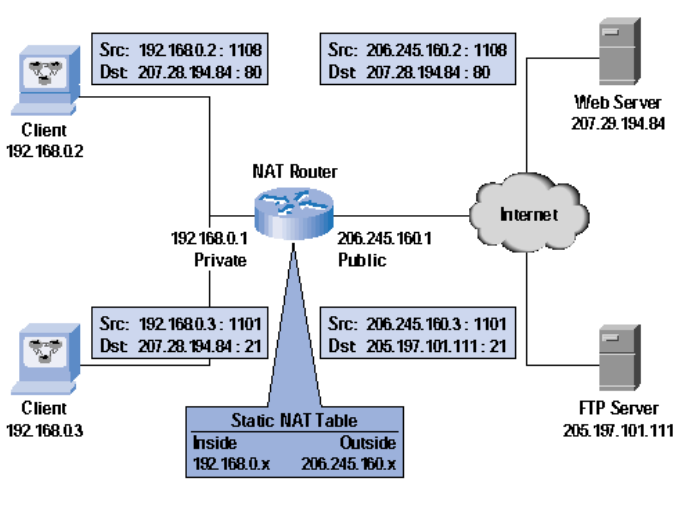
\includegraphics[scale=0.40]{img/static.PNG}
			\caption{Security concepts and relationships\label{fig:2}}
		\end{figure}
		
		\subsection{NAT Dinamico}
			\begin{itemize}
				\item Mapping dinamico tra indirizzi esterni ed indirizzi esterni
				\item Risolve il problema della scarsità degli indirizzi
				\item Richiede Server stateful ( mantiene informazioni di stato dell'utente durante una sessione).
			\end{itemize}
		\textit{NAT Dinamico:\ref{fig:3}}
		\begin{figure}[h!]
			\centering
			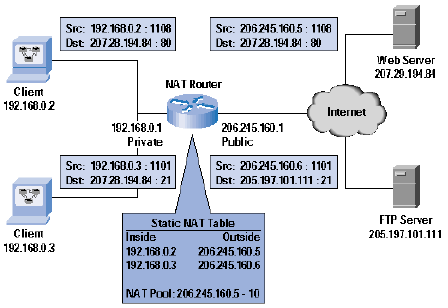
\includegraphics[scale=0.60]{img/dinamic.PNG}
			\caption{Security concepts and relationships\label{fig:3}}
		\end{figure}
		
		\subsection{NAPT: Network Address and Port Translation}
			\begin{itemize}
				\item Mapping dinamico tra indirizzi interni e d esterni \textbf{con porte dinamiche}.
				\item Risolve il problema della scarsità di indirizzi
				\item Richied un serve stateful più complesso rispetto al NAT.
			\end{itemize}
			
			\textit{NAPT:\ref{fig:4}}
			\begin{figure}[h!]
				\centering
				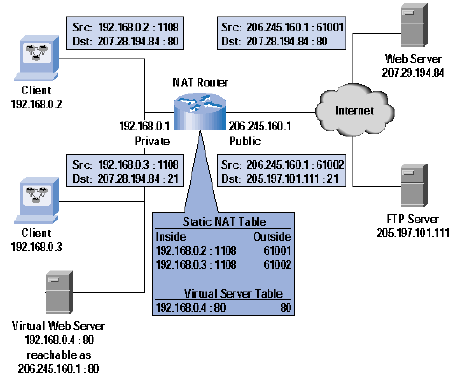
\includegraphics[scale=0.60]{img/natp.PNG}
				\caption{Security concepts and relationships\label{fig:4}}
			\end{figure}
			
			Tuttavia il NAT ha una controindicazione: implica un \textbf{ricalcolo dei checksum} IP e TCP come avviene in IPSec (standard per reti a pacchetto per la sicurezza su reti IP). Le due cose possono \textbf{interferire portando ad un completo blocco delle comunicazioni}. Si hanno problemi sia con la funzione \textbf{AH} (Authentication Header, protocollo per controllo integrità di pacchetto, garantisce authentication pacchetto per pacchetto tramite checksum a chiave simmetrica) sia con la funzione \textbf{ESP} (Encapsulating Security Payload utilizzato per autenitcità confidenzialità e integrità) di IPSEC\\
			
			INSERIRE natipsec\\
			
			\textbf{La soluzione} può essere quella di applicare il NAT e poi IPSEC, o in alternativa eseguirli insieme. Da tenere in considerazione il fatto che un Host dietro a un NAT non può cominciare una comunicazione IPSec (???????). Inoltre la \textbf{co-locazione di NAT e IPSEC è un potenziale pericolo per la sicurezza}. La terza opzione è quella di utilizzare un tunnel IP-over-IP ma è deprecabile.
		\subsection{Basi}
			I pacchetti non routable non sono trasportati in internet (ovvero i router li scartano) poichè il loro indirizzo IP non è univoco. Serve pertanto un traduzione da indirizzi non routable a indirizzi routable: il NAT si occupa di questo.\\
			
			INSERIRE basi\\
			
			Un NAT svolge le seguenti \textbf{operazioni} sia quando arriva un pacchetto sull'interfaccia \textbf{interna} che su quella \textbf{esterna}:
			\begin{itemize}
				\item Si cerca un \textbf{binding} se c'è si trasla il pacchetto e si esegue un \textbf{forward} di quest'ultimo, altrimenti si \textbf{scarta} il pacchetto
				\item Allo scadere di un \textbf{timer} specifico si \textbf{cancella il binding}
			\end{itemize}
		\subsection{NAT RFC 1631 e RFC 2776 }  
			Per quanto riguarda \textbf{RFC 1631} si varia \textbf{solo gli indirizzi IP}, in questo modo tuttavia non risolviamo il problema della scarsità di indirizzi. Infatti il numero di indirizzi necessari è pari al numero di PC che vogliono utilizzare \textit{contemporaneamente} lo stesso protocollo.\\
			
			INSERIRE 1631\\
			
			In RFC 2776 invece, si varia \textbf{sia indirizzi IP che le porte}. In tal modo il numero delle sessione contemporanee (ovvero il numero di bindings contemporanei) è pari circa a 64000 (escludendo le porte ben conosciute.)
		\subsection{NAT binding}
			Per binding intendiamo una relazione: $${IP,proto,port}(int)<=>{IP,Proto,Port}(ext) $$
			In realtà quello che è inteso come bindig è composto da \textbf{Binding + Filter}.
			\begin{itemize}
				\item Il primo associa indirizzo porta interna a un indirizzo porta esterna (realizza la funzione $interno <=> esterno$)
				\item Il secondo decide se e quali pacchetti dall'esterno vanno ritradotti. \textbf{\textit{Attenzione}}: il comportamento del filter genera differenti comportamenti del NAT, alcuni voluti altri no.
			\end{itemize}
			Il binding varia a seconda dei protocolli che utilizziamo, nello specifico parliamo delle differenze che si riscontrano tra \textbf{TCP} e \textbf{UDP} a livello di NAT:
			\begin{itemize}
				\item TCP è \textbf{stateful}, dunque il binding è aggiornato in base ad un timer che varia a seconda dello stato della connessione e della dimensione della CWIN. Per questo protocollo il NAT ha un comportamento \textbf{symmetric} ossia \textbf{binding e filter sono basati sulla stessa quintupla} 
				$$(protocollo, IP, porte sorgente-destinazione) $$
				(Quintupla ?????)\\
				Per questo motivo \textbf{le comunicazioni  devono partire dall'interno} e non è possbili effettuare una callback, quindi PASSIVE FTP (????????). Inoltre il \textbf{demultiplexing è definito a livello TCP} 
				\item UDP è \textbf{stateless}, il binding è basato solo su un timer e sulla conoscenza del comportamento dell'applicazione (informazioni sulle porte utilizzate ad esempio). Il \textbf{demultiplexing} è fatto a \textbf{livello applicazione}, in questo modo una sola applicazioni può utilizzare una sola socket in uscita per due stream diversi con destinatari diversi (a differenza di TCP).
			\end{itemize}
			\textit{\textbf{Abbiamo bisogno di un comportamento diverso del NAT per UDP}}.\\
			Esistono diversi modi di implementare NAT per UDP, queste diverse implementazioni dipendono dalle modalità di esecuzione del Filter. In base a come si comporta NAT alcuni applicativi possono funzionare o meno, in parte o del tutto.
			\subsubsection{Symmetric NAT}
				Funziona esattamente come il symmetric per TCP, non funzioneranno i programmi che hanno bisogno di referral e handover (?????)\\
				
				INSERIRE sym\\
				
			\subsubsection{Full Cone NAT}
			 	\textbf{Il filter non fa niente}. Tutto e tutti potranno raggiungere  il sorgente (compresi malintenzionati, permetto perfino di eseguire un \textbf{port scanning})\\
			 	
			 	INSERIRE cone\\
			 
			 \subsubsection{Restricted Cone NAT}
			 	I\textbf{l Filter è basato sull'IP del destinatario.} Significa che accettiamo comunicazioni da porte diverse purchè abbiano lo stesso IP ( provengano dallo stesso Host). \textbf{Non c'è controllo sul numero di porta}. Questa politica del Filter è restrittiva poichè non permette a programmi come MSN e mulo di funzionare\\
			 	
			 	INSERIRE rest\\
			 	
			 \subsubsection{Port Restricted Cone NAT}
			 	\textbf{Il filter è basato sulla porta del destinatario}. Funzionano tutti i programmi UDP anche se con delle limitazioni.\\
			 	
			 	INSERIRE port\\
			 	
			 \subsubsection{NAT - STUN}
			 	\textit{Come può un'applicazione conoscere il tipo di NAT ?}\newline
			 	Si utilizza un protocollo chiamato \textbf{STUN}, un protocollo \textbf{request-reply}. Esso permette alle applicazioni in esecuzione su un computer di scoprire la presenza ed i tipi di NAT e firewall che si interpongono tra il computer e la rete pubblica. Permette inoltre a questi computer di conoscere gli indirizzi IP e le porte con cui il dispositivo NAT li sta rendendo visibili sulla rete pubblica. \textbf{Ha a disposizione due porte sul client e due porte e due indirizzi ip sul server}\\
			 	STUN non grarantisce una conoscenza accurata, infatti il \textbf{NAT può essere non deterministico}, ossia cambiare il comportamento a seconda della disponibilità delle risorse. Un altro problema si riscontra nella possibilità che ci siano più NAT nel percorso sorgente-destinazione, in questo caso la classificazione non è rigorosa e il comportamento imprevedibile (Il secondo livello di NAT potrebbe non avere lo stesso comportamento del primo)
		\subsection{NAT: ulteriori classificazioni}
			I NAT possono essere classificati in base a tre parametri:
			\begin{itemize}
				\item Come viene fatto il \textbf{binding}.
				\item Come vengono \textbf{aggiornati i filters.}
				\item Quando si riavviano i \textbf{timers.}
			\end{itemize}
			\subsubsection{In base al Binding}
				\begin{itemize}
					\item \textbf{Endpoint}: il NAT riusa il binding per tutte le sessioni provenienti da stesso IP/PORTA, IP/PORTA esterni non vengono valutati (\textbf{come full cone NAT})
					\item \textbf{Endpoint}:Il NAT riusa il binding per tutte le sessioni provenienti dalla stesso IP/porta verso lo stesso IP esterno (la porta non si considera).
					\textbf{E’ come un Restricted Cone NAT.}
					\item \textbf{Endpoint address and port dependent}: come symmetric NAT.  	
				\end{itemize}
			\subsubsection{In base al Port Binding}
				\begin{itemize}
					\item \textbf{Port preservation}: Il NAT tenta di mantenere la porta di origine. Se due Host interni utilizzano la stessa porta di origine uno l'avrà cambiata l'altro no.
					\item \textbf{Port overloading}: Il NAT fa port preservation in modo aggressivo, un secondo tentativo di binding fa scadere il binding esistente
					\item \textbf{Port}: ??????
				\end{itemize}
			\subsubsection{In base al Timer Refresh}
				\begin{itemize}
					\item \textbf{Bidirectional}: il timer è aggiornato dai pacchetti in entrambe le direzioni.
					\item \textbf{Outbound}: Solo pacchetti interno verso l'esterno rinfrescano i timer. Risulta necessario usare un \textbf{keep alive}. Inoltre il timer potrebbe essere per session o per binding ( nel caso di riuso del binding per piu sessioni)
					\item \textbf{Inbound}: solo i pacchetti dall'esterno verso l'interno rinfrescano il timer, anche in questo caso c'è bisogno di un keep- alive
					\item \textbf{Transport protocol state}: come in TCP ma si possono usare altre informazioni (da la possibilità di fare attacchi DOS).
				\end{itemize}
			\subsubsection{In base all'External Filtering }
				\begin{itemize}
					\item \textbf{Endpoint independent}: non filtra o scarta pacchetti (full cone)
					\item \textbf{Endpoint address dependent}: Filtra i pacchetti che non provengono dall'IP originario del binding (restricted cone).
					\item \textbf{Endpoint address and port dependent}:  Filtra i pacchetti che non provengono dall'IP/porta originario del binding (port restricted cone o symmetric).
				\end{itemize}
			\subsection{Considerazioni}
				Per quanto riguarda le \textbf{applicazioni p2p} esse tendono ad aggirare il NAT ma così facendo creano spesso problemi di sicurezza. Per quanto riguarda ICMP rischia di fallire per lo stesso motivo di IPSEC (nel payload sono spesso contenute info su IP e porta originante). Rispetto all'\textbf{IP fragmentation} il problema è quello di ricostruire i pacchetti (o almeno mantenute informazioni sul primo pacchetto), perchè nei frammenti successivi \textbf{manca header UDP/TCP}, ma \textbf{potrebbe essere un attacco a frammentazione}. Inoltre il primo pacchetto può arrivare fuori sequenza. Una soluzione è quella di provare a configurare il nat in modo che esso stesso modifichi il contenuto del payload.
			\subsubsection{NAT: UPnP e IGD}
				\textbf{Universal Plug n Play}: Set di protocolli per la definizione  e l'annuncio di device e servizi. Un dispositivo compatibile UPnP può unirsi dinamicamente ad una rete, ottenendo un indirizzo IP, annunciare il suo nome, trasmettere le proprie capacità su richiesta e venire a conoscenza della presenza e delle capacità degli altri device della rete.\\
				L'\textbf{Internet Gateway Device (IGD) } permete ad un device UPnP di scoprire l'indirizzo esterno di un NAT e di creare filters e bindings per i suoi servizi in modo automatico. In questo modo le porte sono aperte in modo incontrollato  e potrebbero sovrascrivere i binding esistenti... come per la porta 80 (implementato in Windows).
				
				
				
		
			
			
				
			
			
			
			 
						
		
		
		
			
		
				 
\end{document}